% Global document settings
\documentclass[10pt]{article}

% Packages
\usepackage{tgtermes}
\usepackage{graphicx}
\usepackage{natbib}
\usepackage{authblk}
\usepackage{array}
\usepackage{colortbl}
\usepackage{tocloft}
\usepackage{xcolor}
\usepackage{siunitx}
\usepackage{setspace}
\usepackage{listings}
\usepackage{caption}
\usepackage[T1]{fontenc}
\usepackage[nottoc]{tocbibind}
\usepackage[breaklinks]{hyperref}
\usepackage[font=small,skip=7pt]{caption}

% Custom colours
\definecolor{codegreen}{rgb}{0,0.6,0}
\definecolor{codegray}{rgb}{0.5,0.5,0.5}
\definecolor{codepurple}{rgb}{0.58,0,0.82}
\definecolor{backcolour}{rgb}{0.95,0.95,0.92}

% Listing styles
\lstdefinestyle{mystyle}{
  backgroundcolor=\color{backcolour},
  commentstyle=\color{codegreen},
  keywordstyle=\color{purple},
  numberstyle=\tiny\color{codegray},
  stringstyle=\color{codepurple},
  basicstyle=\ttfamily\footnotesize,
  breakatwhitespace=false,
  breaklines=true,
  captionpos=b,
  keepspaces=true,
  numbers=left,
  numbersep=5pt,
  showspaces=false,
  showstringspaces=true,
  showtabs=false,
  tabsize=2
  }
  \lstset{style=mystyle}

  % Custom commands
  \renewcommand\cftsecafterpnum{\vskip8pt}
  \renewcommand{\lstlistlistingname}{List of \lstlistingname s}
  \renewcommand{\bibsection}{\section*{Bibliography}}
  \renewcommand{\contentsname}{Table of Contents}
  \renewcommand{\bibsection}{\section{\bibname}}
  \renewcommand{\cftsecleader}{\cftdotfill{\cftdotsep}}

  % Custom settings
  \captionsetup{justification=centering}
  \PassOptionsToPackage{hyphens}{url}
  \urlstyle{same}
  \def\Urlmuskip{0mu}
  \def\UrlBreaks{\do\/\do-}
  \hypersetup{
    colorlinks = true,
    urlcolor = blue,
    linkcolor = black,
    citecolor = black,
  breaklinks=true,
  pdfpagemode=UseOutlines,
  bookmarksopen=true,
  bookmarksopenlevel=2,
  bookmarksnumbered=true
  }

  \title{\textbf{Evaluating the Quality of Life Concept:} \\ A Critical Examination of its Application and Value in Understanding Mental Health Burdens}
  \author[ ]{Daniel Burger}
  \affil[ ]{\textbf{King’s College London}}
  \affil[ ]{\href{mailto:public@danielburger.online}{public@danielburger.online}}
  \date{\textit{13. June 2023}}

\begin{document}
\pagenumbering{roman}
\counterwithin{lstlisting}{section}
\counterwithin{figure}{section}
\counterwithin{table}{section}

\maketitle
\thispagestyle{empty}

\begin{sloppypar} % For better line breaks
  \begin{abstract}
    This essay critically examines the Quality of Life (QoL) concept and its applications in mental health research and practice. With its multidimensional construct and inherent subjectivity, QoL provides a comprehensive measure of an individual’s mental state, transcending traditional symptom-focused metrics. Tools like the Quality of Life Enjoyment and Satisfaction Questionnaire (Q-LES-Q) offer nuanced insights into patients’ subjective well-being. QoL measures play a vital role in global health burden estimations. However, the variability and potential bias in self-reported QoL measures, along with issues of cross-cultural comparability, pose significant challenges. While QoL offers a beneficial lens through which to comprehend and tackle the weight of mental health issues, the essay finishes by highlighting the necessity for a subtly differentiated interpretation of QoL assessments. It argues for sustained investigation to fine-tune these methodologies and confirm their effectiveness.
  \end{abstract}
  \pagebreak

  \pagenumbering{Roman}
  \tableofcontents
  \pagebreak

  \listoffigures
  \pagebreak

  \listoftables
  \pagebreak


  % Double spacing for feedback
  \doublespacing

  \pagenumbering{arabic}
  \section{Introduction} \label{sec:introduction}
  Quality of Life (QoL) is a broad concept that considers many aspects of life, such as physical health, psychological condition, social interactions, personal beliefs, and surroundings. It has become quite a big deal in health research and clinical care, especially mental health. As the World Health Organization outlines, QoL is a highly subjective matter heavily influenced by an individual’s cultural background, moral values, and personal aspirations. This makes it a holistic way to look at a person’s overall well-being \citep{harper_development_1998}.

  This concept is practically operationalised through assessment tools such as the WHOQOL questionnaire, as illustrated in \autoref{fig:qol-questionnaire}. QoL measures extend beyond the clinical symptoms to capture the full spectrum of an individual’s life experiences, enhancing our understanding of mental health burdens.

  \begin{figure}[ht] \centering 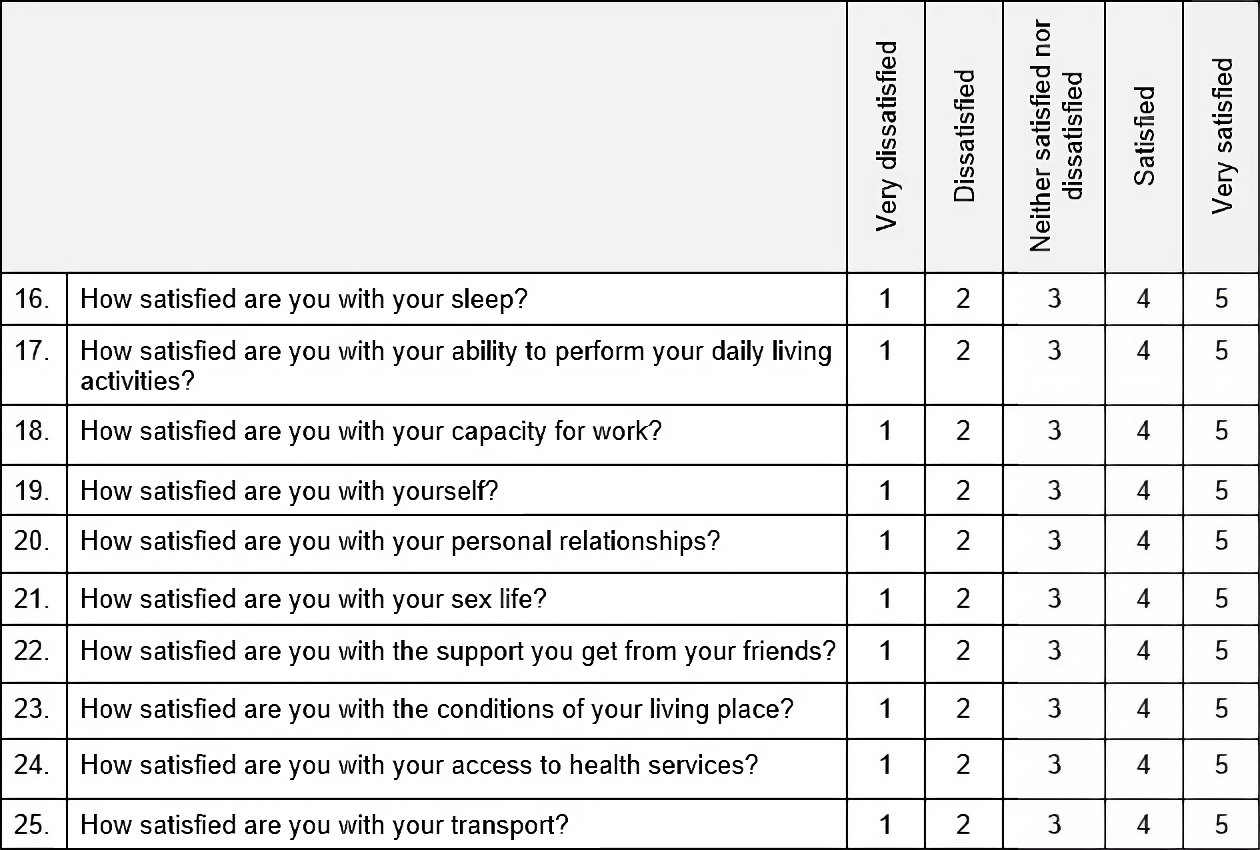
\includegraphics[width=\textwidth]{figures/qol-questionnaire.png} \caption[Screenshot of example questions of a QoL questionnaire.]{Screenshot of example questions of a QoL questionnaire \citep{harper_development_1998}.} \label{fig:qol-questionnaire} \end{figure}

  \newpage

  QoL has broad applications across public health, psychiatry, and applied neuroscience. For example, in psychiatry, QoL metrics supplement traditional outcome measures such as symptom severity, contributing to shared decision-making processes in clinical practice and guiding policy-making at a population level. Applied neuroscience, meanwhile, uses QoL to connect the biological underpinnings of mental disorders with subjective patient experiences, as evidenced by studies indicating significant neurological implications on life satisfaction in disorders like depression \citep{zhang_brain_2016}.

  However, despite its broad applicability, the concept of QoL has its criticisms and limitations. The subsequent chapters will critically examine the benefits and drawbacks of the QoL concept in understanding mental health burdens.

  \section{Benefits of the Quality of Life Concept}
  \label{sec:benefits}

  The concept of QoL serves as a potent tool in mental health research and practice, offering benefits that address some of the limitations inherent in traditional clinical measures. This chapter explores these advantages, critically reviewing the empirical literature to provide a nuanced perspective.

  \subsection{More Holistic Understanding of Patient Well-being}
  \label{subsec:holistic}
  One of the most significant benefits of the QoL concept is its broader, more comprehensive perspective on patient well-being. Traditionally, the assessment of mental health disorders relied heavily on symptomatic evaluations. However, the subjective experience of mental health is far more complex and extends beyond the presence or absence of symptoms. QoL assessments capture a range of factors that influence a person’s well-being, including physical health, psychological status, social relationships, and environment.

  Studies suggest that these factors can often deviate from clinical symptoms, revealing unique aspects of a patient’s experience that may otherwise remain unnoticed. For example, a study on patients with schizophrenia found that while clinical symptom severity decreased over time, many patients reported no improvement in their QoL \citep{eack_quality_2007}. These findings underscore the value of QoL measures in painting a more comprehensive picture of patient well-being.

  \subsection{Enhanced Patient-Centered Care}
  \label{subsec:patient-centered}
  The QoL concept also supports a patient-centred approach in mental health care, aligning treatment goals with patients’ unique needs and life contexts. Patient-centred care emphasises active patient participation in the treatment process and decision-making, an approach associated with improved treatment adherence and patient satisfaction \citep{dwamena_interventions_2012}.

  QoL measures can guide the delivery of personalised interventions by highlighting areas that matter most to the patient. For instance, the Quality of Life Enjoyment and Satisfaction Questionnaire (Q-LES-Q), as shown in \autoref{fig:q-les}, has been used to obtain sensitive measures of enjoyment and satisfaction in various areas of daily functioning. This tool captures the patient’s experience beyond the severity of illness or depression, potentially informing more personalised therapeutic approaches \citep{endicott_quality_1993}. This underscores the utility of QoL measures in tailoring interventions that resonate with patients’ life contexts and goals.

  \begin{figure}[ht]
    \centering
    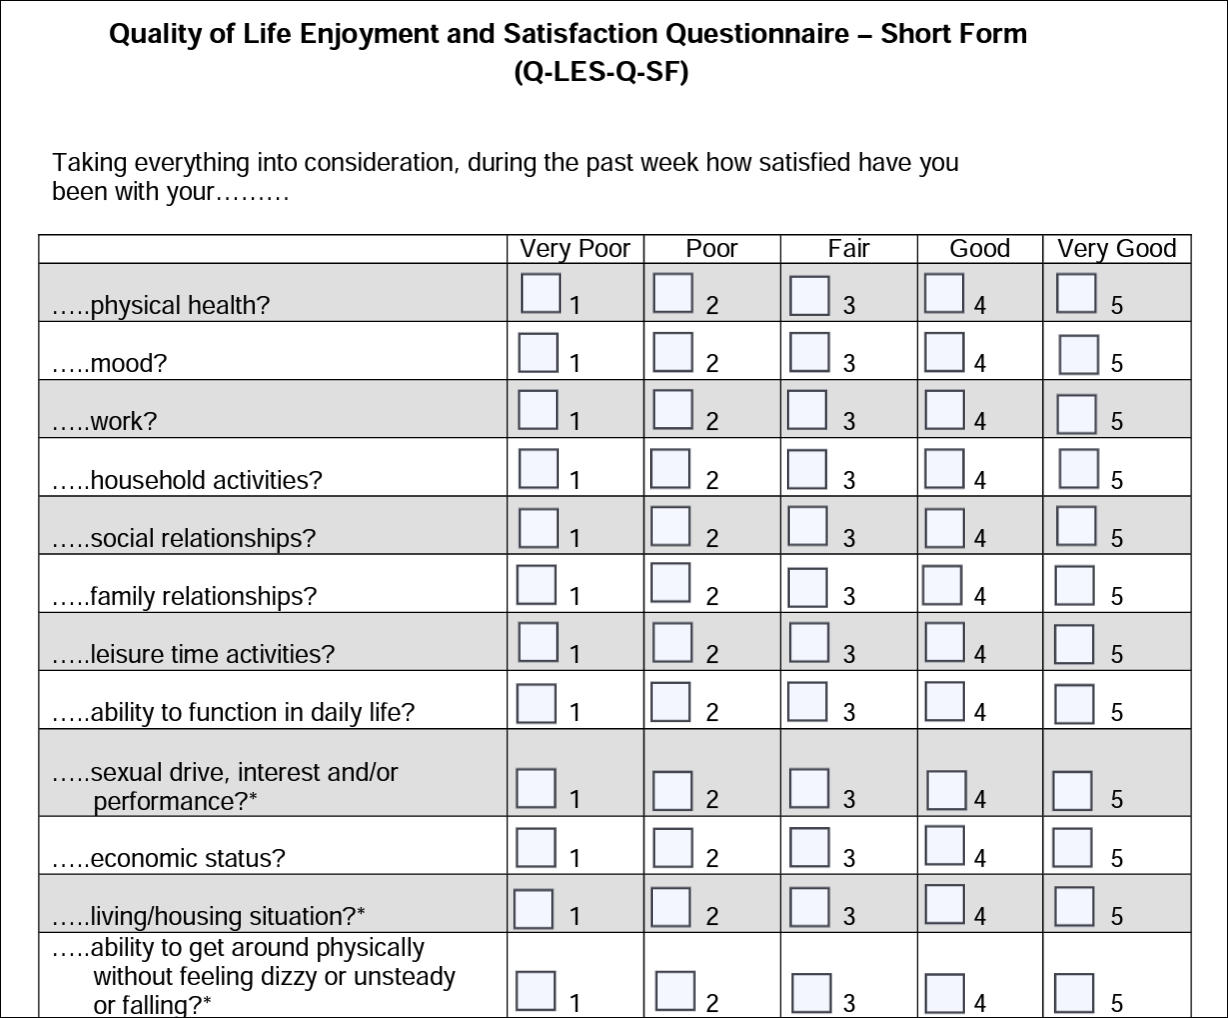
\includegraphics[width=\textwidth]{figures/q-les.png}
    \caption[Screenshot of example questions of the Quality of Life Enjoyment and Satisfaction Questionnaire (Q-LES-Q) questionnaire.]{Screenshot of example questions of the Quality of Life Enjoyment and Satisfaction Questionnaire (Q-LES-Q) questionnaire \citep{endicott_quality_1993}.}
    \label{fig:q-les}
  \end{figure}

  \subsection{Insight into Population Health and Informing Health Policy}
  \label{subsec:population-health}
  QoL metrics offer a comprehensive view of population health and can guide health policies. This is shown in \autoref{fig:qol-map}, which uses QoL to illustrate the World Happiness Report. By incorporating QoL indicators, mental health research can reveal disparities, track changes over time, and assess the impact of interventions or policy changes at a population level.
  For example, the Global Burden of Disease Study \citeyearpar{gbd_2017_disease_and_injury_incidence_and_prevalence_collaborators_global_2018} provides a systematic analysis of the incidence, prevalence, and years lived with disability for numerous diseases and injuries worldwide, including mental disorders \citep{gbd_2017_disease_and_injury_incidence_and_prevalence_collaborators_global_2018}. This comprehensive report contributes valuable data to inform global mental health policies by accounting for these factors. This example underscores the potential of QoL metrics to influence policy-making, highlighting the broader societal value of the QoL concept.

  \begin{figure}[ht]
    \centering
    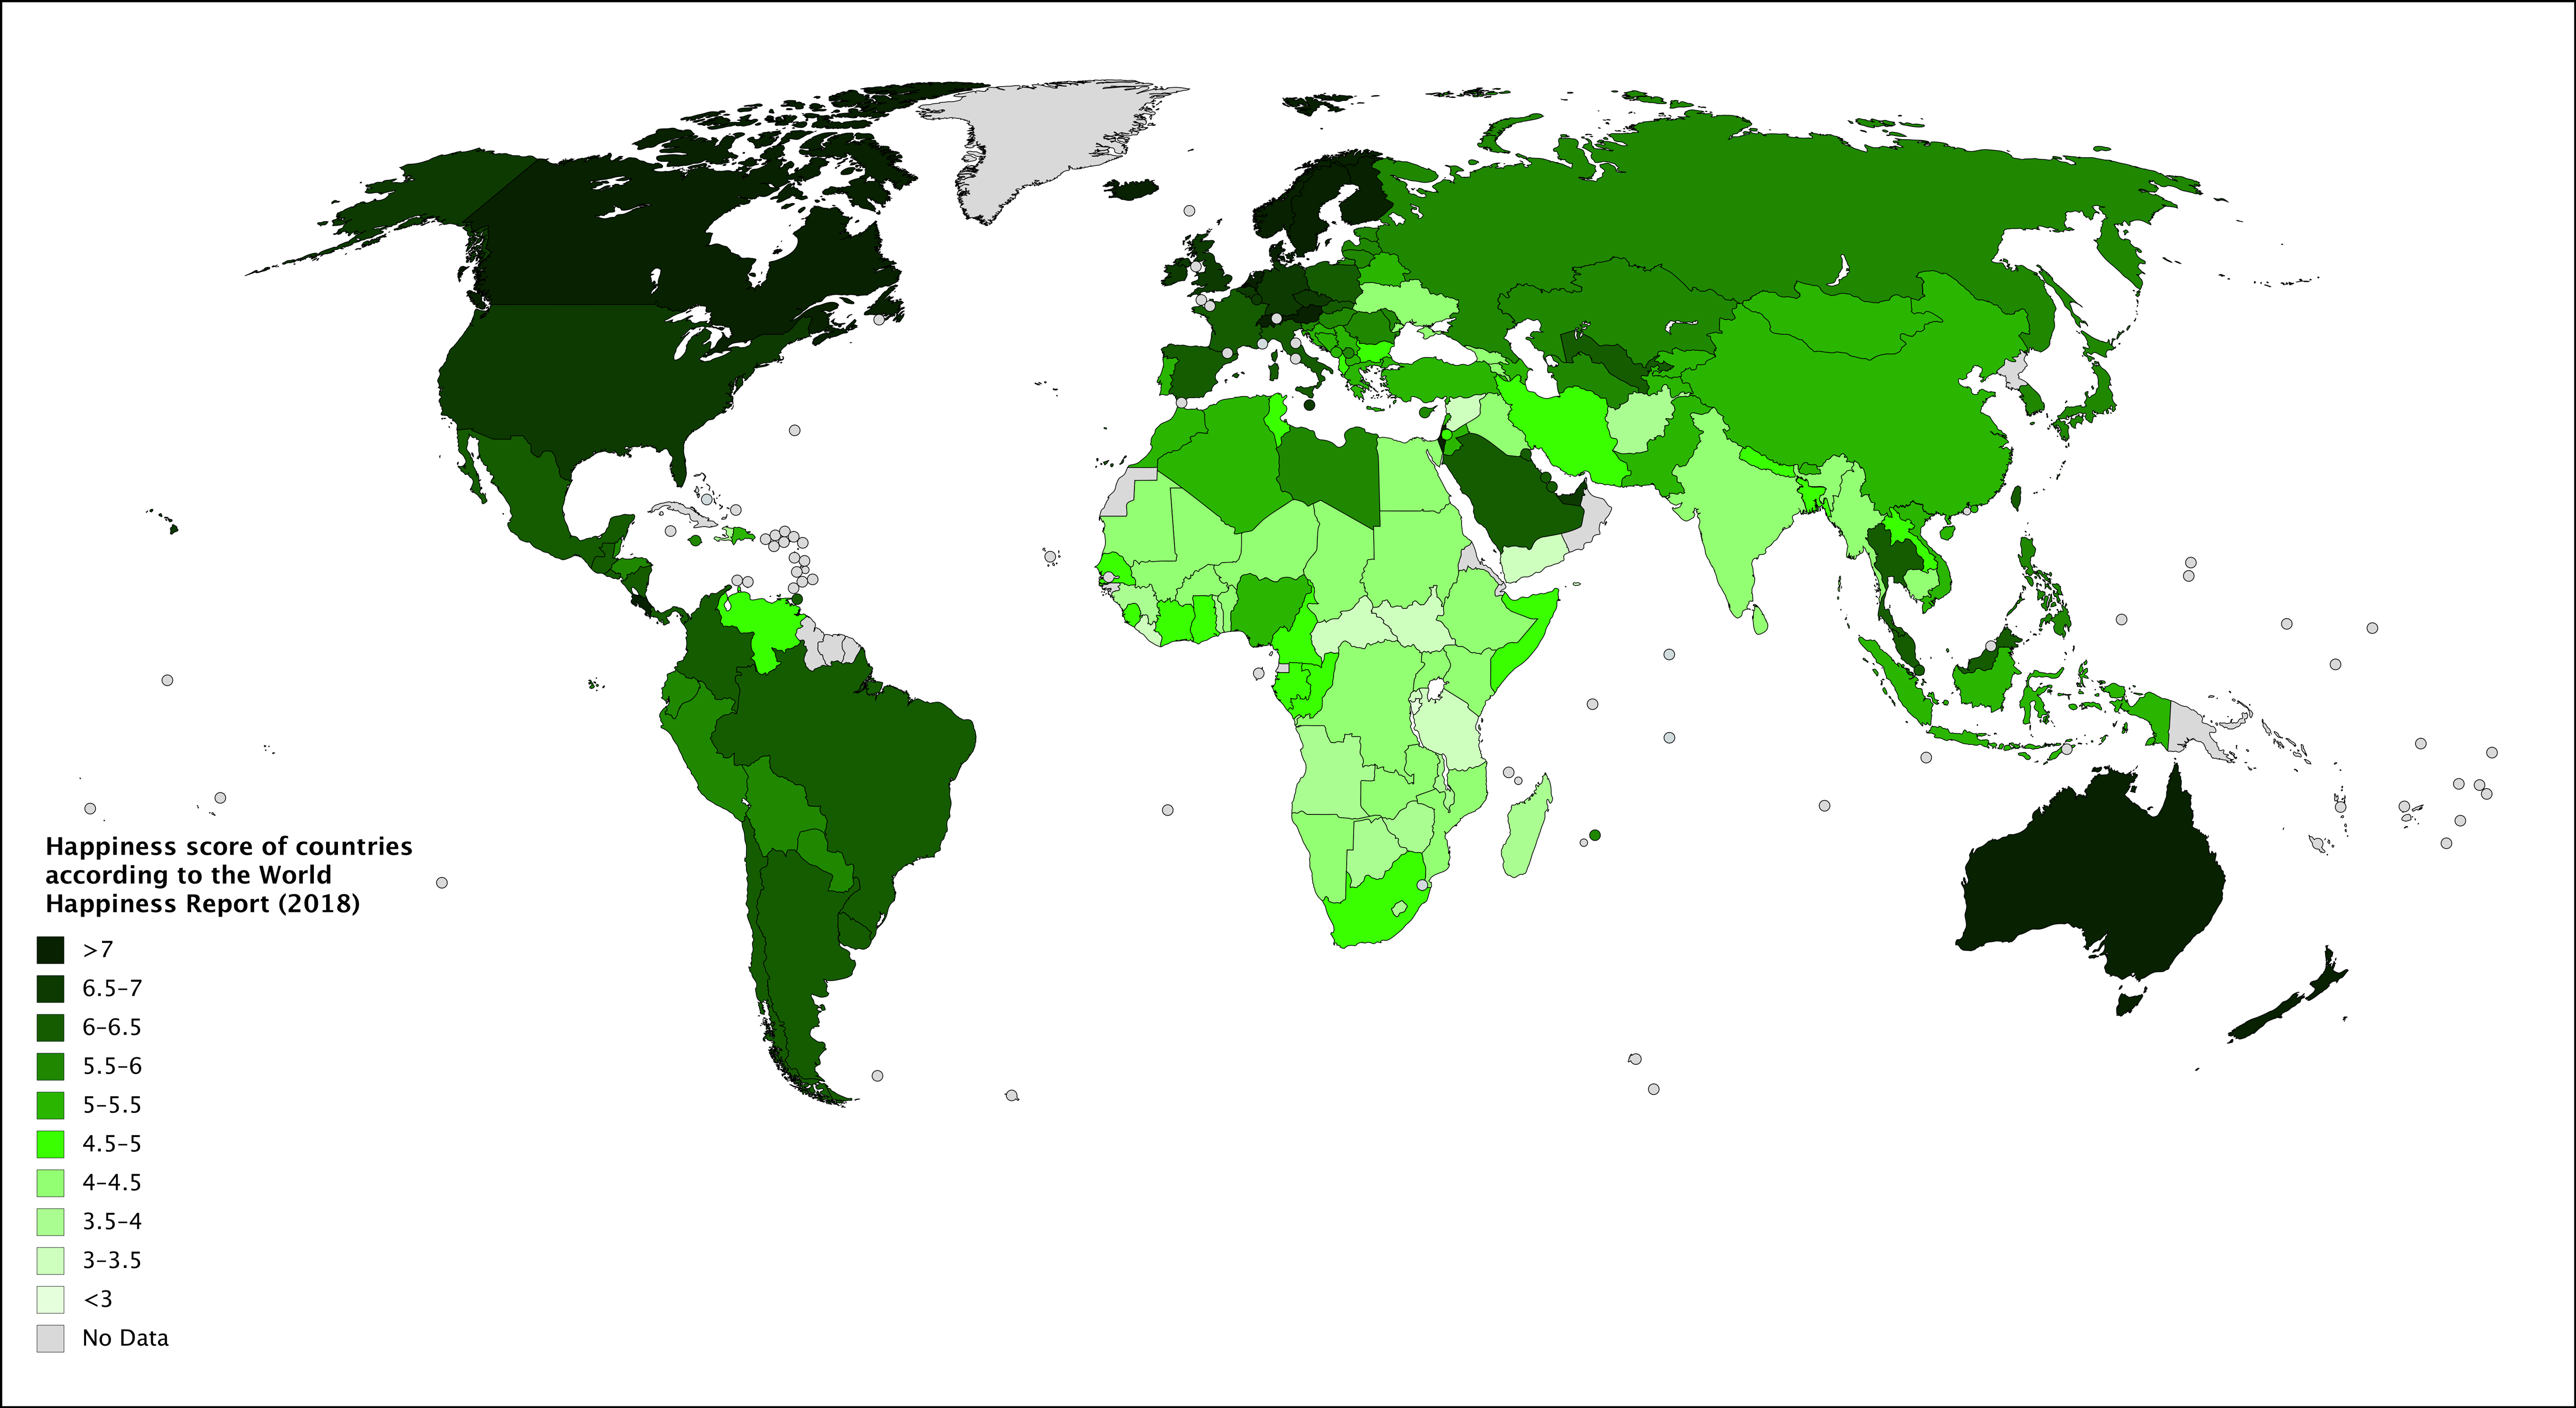
\includegraphics[width=\textwidth]{figures/qol-world.png}
    \caption[A world map displaying the happiness levels of countries based on their QoL scores as reported in the 2018 World Happiness Report.]{A world map displaying the happiness levels of countries based on their QoL scores as reported in the 2018 World Happiness Report \citep{helliwell_world_2018}.}
    \label{fig:qol-map}
  \end{figure}

  \section{Limitations of the Quality of Life Concept}
  \label{sec:limitations}

  As beneficial as the QoL concept is in understanding mental health burdens, it is not without limitations. This chapter discusses some drawbacks, critically engaging with recent research to provide an unbiased view of the concept’s utility.

  \subsection{Subjectivity and Variability}
  \label{subsec:subjectivity}
  QoL is subjective and varies between individuals due to differences in personal values, cultural background, and life circumstances. This subjectivity makes comparing QoL scores across different individuals or groups challenging and can lead to misinterpretations or biases \citep{skevington_expecting_2012}.

  \subsection{Measurement Challenges}
  \label{subsec:measurement}
  Linked to its subjectivity is the challenge of accurately measuring QoL. Several instruments exist to assess QoL, each with varying sensitivity, reliability, and validity levels. For instance, the WHOQOL-BREF and the Q-LES-Q are widely used. However, they emphasise different aspects of QoL, as shown in \autoref{tab:overview-QoL-tools}, leading to potential inconsistencies between the measures \citep{endicott_quality_1993,harper_development_1998}. Moreover, these measures rely on self-reporting, which can be influenced by temporary mood states, recall biases, or social desirability \citep{bowling_just_2005}.

  \vspace{10pt} % Increase vertical spacing before table
  \begin{table}[ht]
    \centering
    \renewcommand{\arraystretch}{1.5}
    \setlength{\tabcolsep}{12pt}
    \resizebox{\columnwidth}{!}{%
      \begin{tabular}{|>{\hspace{0pt}}m{0.3\linewidth}|>{\hspace{0pt}}m{0.35\linewidth}|>{\hspace{0pt}}m{0.35\linewidth}|}
        \hline
        \rowcolor[HTML]{D3D3D3} % Grey color for the heading row
        {\color[HTML]{000000} \textbf{}}                       & {\color[HTML]{000000} \textbf{WHOQOL-BREF}}                                                     & {\color[HTML]{000000} \textbf{Q-LES-Q}}                                                                                                              \\ \hline
        \rowcolor[HTML]{FFFFFF}
        {\color[HTML]{000000} Primary Domain Focus}            & {\color[HTML]{000000} Physical health, Psychological health, Social relationships, environment} & {\color[HTML]{000000} Physical health, Mood level, Work functioning, Household duties, Leisure activities, Social relationships, General activities} \\ \hline
        \rowcolor[HTML]{FFFFFF}
        {\color[HTML]{000000} Number of Items}                 & {\color[HTML]{000000} 26 items}                                                                 & {\color[HTML]{000000} 93 items}                                                                                                                      \\ \hline
        \rowcolor[HTML]{FFFFFF}
        {\color[HTML]{000000} Scaling}                         & {\color[HTML]{000000} 5-point Likert scale}                                                     & {\color[HTML]{000000} 5-point Likert scale}                                                                                                          \\ \hline
        \rowcolor[HTML]{FFFFFF}
        {\color[HTML]{000000} Sensitivity to Change}           & {\color[HTML]{000000} High/Low (depends on research)}                                           & {\color[HTML]{000000} High/Low (depends on research)}                                                                                                \\ \hline
        \rowcolor[HTML]{FFFFFF}
        {\color[HTML]{000000} Cross-Cultural Adaptability}     & {\color[HTML]{000000} High (developed by WHO, used globally)}                                   & {\color[HTML]{000000} Varies (can be adapted, but not as universal as WHOQOL-BREF)}                                                                  \\ \hline
        \rowcolor[HTML]{FFFFFF}
        {\color[HTML]{000000} Complexity (Time to Administer)} & {\color[HTML]{000000} Moderate}                                                                 & {\color[HTML]{000000} High due to more items}                                                                                                        \\ \hline
      \end{tabular}%
    }
    \caption{Comparison of the WHOQOL-BREF and Q-LES-Q quality of life questionnaires.}
    \label{tab:overview-QoL-tools}
  \end{table}



  \subsection{Lack of Standardisation}
  \label{subsec:standardisation}
  Another downside to the QoL concept is its need for more definition and measurement standardisation. While organisations like WHO have proposed definitions, many variants exist, leading to a need for more consensus in the literature. This fragmentation can pose difficulties in comparing studies, implementing interventions, or formulating policies based on QoL \citep{matarazzo_behavioral_1980}.

  \subsection{Complexity and Indirectness}
  \label{subsec:complexity}
  Finally, the QoL concept introduces complexity to mental health assessments and interventions. Given its broad and multifaceted nature, it can be challenging to pinpoint specific factors influencing QoL and to design interventions that address these elements. Moreover, making a direct link between specific treatments or interventions and changes in QoL can be more complex than symptom-focused measures. This complexity necessitates a careful, nuanced approach to using and interpreting QoL measures in mental health contexts.

  In summary, while the QoL concept provides a rich, holistic view of mental health burdens, it also introduces several complexities and challenges. Its value should therefore be evaluated alongside these considerations, seeking to maximise its strengths while acknowledging and addressing its limitations.

  \section{Summary}
  \label{sec:summary}

  The QoL concept holds significant potential in deepening our understanding of mental health burdens, offering a nuanced, person-centred perspective beyond traditional symptom-based measures. However, its application in psychiatry, mental health, and applied neuroscience is not without challenges.

  This essay has critically discussed the benefits and drawbacks of the QoL concept, grounding the discussion in contemporary research to provide a balanced view. Among the key benefits of the QoL concept includes its capacity to illuminate the lived experiences of individuals with mental health conditions, enhancing personalised care by providing a platform to capture patients’ unique needs and life contexts \citep{dwamena_interventions_2012,endicott_quality_1993}. Furthermore, QoL indicators can significantly contribute to understanding population health, helping inform health policies on a broader scale \citep{gbd_2017_disease_and_injury_incidence_and_prevalence_collaborators_global_2018}.

  Nevertheless, the QoL concept has shortcomings. Its inherent subjectivity and variability can pose challenges in comparing QoL scores across individuals or groups \citep{skevington_expecting_2012}. Measurement of QoL presents its own set of difficulties, especially given the reliance on self-report measures that could be influenced by factors such as mood states, recall biases, or social desirability \citep{bowling_just_2005}. The lack of standardisation in QoL definition and measurement can create difficulties in comparing studies or formulating policies \citep{matarazzo_behavioral_1980}. Lastly, the complexity and indirectness of QoL measures necessitate a careful, nuanced approach to their use and interpretation in mental health contexts.

  Moving forward, there is considerable scope for further research to enhance our understanding and utilisation of the QoL construct. Potential avenues include mitigating biases in self-reported QoL measures, such as developing standardisation strategies to account for individual differences in QoL perceptions and experiences. Furthermore, the cross-cultural applicability of QoL deserves further investigation. Research can contribute towards a more nuanced understanding of this complex construct by conducting comparative studies across different cultural groups, refining QoL measures to capture culturally-specific aspects of well-being better, or developing new QoL instruments tailored to specific cultural contexts.

  In conclusion, the QoL concept offers a valuable tool to understand and address mental health burdens. Its strengths and limitations should be carefully considered, advocating for its judicious use alongside other measures to provide a comprehensive, balanced understanding of mental health. As we refine our understanding and measurement of QoL, we can better serve the diverse needs of individuals with mental health conditions and contribute towards a more holistic, person-centred approach to mental health research and practice.

  \pagebreak
  \singlespacing % No need for double spacing in the references
  \bibliographystyle{references/custom-apa}
  \bibliography{references/bibliography}

\end{sloppypar}
\end{document}